\documentclass{article}
\usepackage[utf8]{inputenc}
\usepackage{enumitem}
\usepackage{enumerate}
\usepackage{amsmath}
\usepackage{graphicx}
\usepackage[demo]{graphicx}
\usepackage{subcaption}

\usepackage{natbib}
\usepackage{titlesec}

\titleformat{\section}
{\normalfont\Large\bfseries}{\thesection}{1em}{}[{\titlerule[0.8pt]}]

\title{ECON7103 HW3}
\author{Sedat Ors}
\date{January 30th}

\begin{document}

\maketitle

\section{Stata}

\begin{enumerate}
\item

\begin{itemize}
\item a)
\vspace{0.5cm}
Let's take the log of both sides  $y_i$ = $e^{\alpha}{\delta^{d_i}}{z_i^{\gamma}}{e^{\eta_i}}$ 

$ln{y_i}$ = ${\alpha}{lne} +{d_i}{ln\delta} + {\gamma}{z_i} +{\eta_i}{lne}$ where lne = 1

So $ln{y_i}$ = ${\alpha} +{d_i}{ln\delta} + {\gamma}{z_i} +{\eta_i}$
\vspace{0.5cm}
\item b)
$\delta$ menans percentage change. if we increase $\delta$ 1 percent ${y_i}$ changes 1 percent. 
But if we need to interpret for the retrofit program, it shows the effectiveness of treatment program. if ${d_i} = $1 
it means everybody treated in the group, if not $\delta$ =0. 
\vspace{0.5cm}
\item c)
when we take derivative of equation above according to the ${d_i}$,

${\frac{1}{y_i}}{\frac{\Delta{y_i}}{\Delta{d_i}}} = ln\delta$

${\frac{\Delta{y_i}} {\Delta{d_i}}}=  l{n\delta}{y_i}$
\vspace{0.5cm}

Note: I can not understand that whether ${\delta}$ is a function of ${d_i}$ or not. I assume ${\delta}$ not dependant variable of ${d_i}$.The average marginal effect (AME) is a measure of the average change in the outcome of a dependent variable (y) resulting from a change in the independent variable (x), holding all other variables constant. The AME represents the average treatment effect of the change in x on y for a given sample or population. It provides insight into the overall relationship between x and y, and can help to identify the most important predictors of the outcome. So, if we change ${d_i}$ 1 unit, ${y_i}$ change $ln\delta$

\vspace{0.5cm}
\item d)
\vspace{0.5cm}
Let's take the derivative of the equation above,

${\frac{1}{y_i}}{\frac{\Delta{y_i}}{\Delta{z_i}}} = {\gamma}{\frac{1}{z_i}}$

${\frac{\Delta{y_i}}{\Delta{d_i}} = {\gamma}{\frac{y_i}{z_i}}} $

when if change ${z_i}$ 1 unit, ${y_i}$ change ${\gamma}{\frac{1}{z_i}}$

\item e)
\noindent See Figure 1 - table 1 
\begin{figure}[]
    \centering
     \includegraphics{HW3Q5.png}
    \caption{Electricity usage}
    \label{tab:question3}
\end{figure}

\item f)
\noindent See Figure 2
\begin{figure}[]
    \centering
     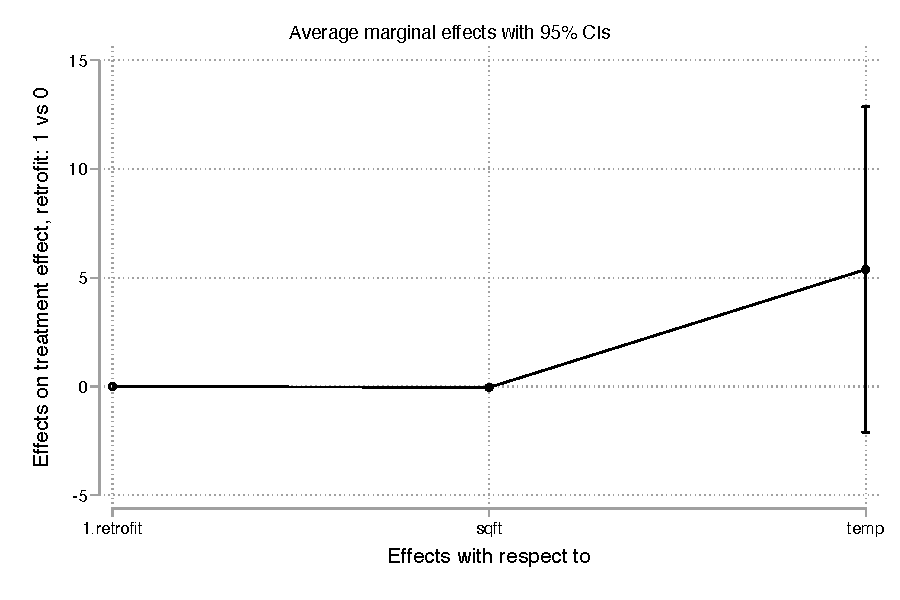
\includegraphics{HW3Q6.pdf}
    \caption{}
    \label{tab:question3}
\end{figure}

\end {itemize}

\end{enumerate}

\end{document}

